% !Mode:: "TeX:UTF-8"

\chapter{红外无人机目标检测算法轻量化}

\section{引言}
对于实际的红外无人机目标检测任务,任务环境常常是野外开阔地带,因此
检测算法常常需要在移动设备上运行,而对于移动端嵌入式设备,硬件的运算能力和成本都十分有限,因此对算法的内存占用和运行时间有更高的要求。也就是在保证检测精度的同时也要保证实时性,这就需要对算法进行一定程度的轻量化,降低算法的内存占用和运行时间,使得移动端设备也可以实时实现红外无人机目标检测。
本章将在上文提到的算法基础上,应用ghost模块对算法模型进行轻量化,并且在PC端和移动端NVIDIA AGX XAVIER设备上进行算法的性能测试,并对实验结果进行分析。

\section{网络结构改进}
Ghost 模块是一种替代传统CNN中的卷积操作并且获得更快速度和更小模型体积的方案。通过对比分析ResNet-50网络第一个残差组(Residual group)输出的特征图可视化结果,发现一些特征图高度相似。如果按照传统的思考方式,可能认为这些相似的特征图存在冗余,是多余信息,想办法避免产生这些高度相似的特征图。而ghost模块另辟蹊径,选择以一种更简单的操作来生成相同数量的特征图,从而实现更快速高效的检测。

\subsection{Ghost模块思想}
典型的卷积计算过程如图\ref{conv}所示,所有的输入逐一经过卷积运算后生成新的特征图。这里的每一个输出张量都是一个由卷积核运算产生的特征图。但是这些特征图中可能有些特征图相似度较高,因此可以认为两张或几张比较相似的特征图是产生于几次同样代价的卷积是一种浪费。

\begin{figure}[htbp]
    \centering
    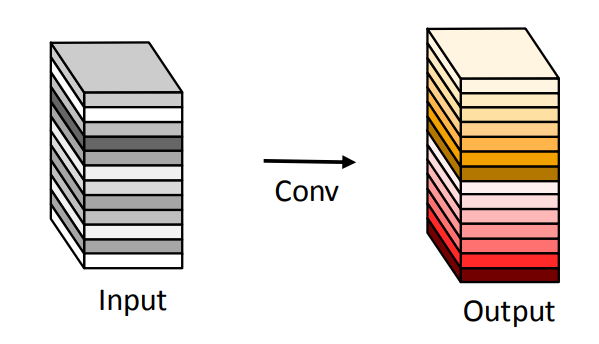
\includegraphics[width = 0.8\textwidth]{传统卷积.png}
    \caption{传统卷积示意图}
    \label{conv}
\end{figure}

如图\ref{identical}所示,每次卷积的所有输出中,可以找到一些相互之间相似度较高的特征图。设图中的A, A’、B B’相似度较高,可以设计一种计算方法替代生成A’和B’的卷积运算,从而达到减小计算量的目的。

\begin{figure}[htbp]
    \centering
    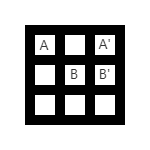
\includegraphics[width = 0.8\textwidth]{重复特征图.png}
    \caption{重复特征图示意图}
    \label{identical}
\end{figure}

\begin{figure}[htbp]
    \centering
    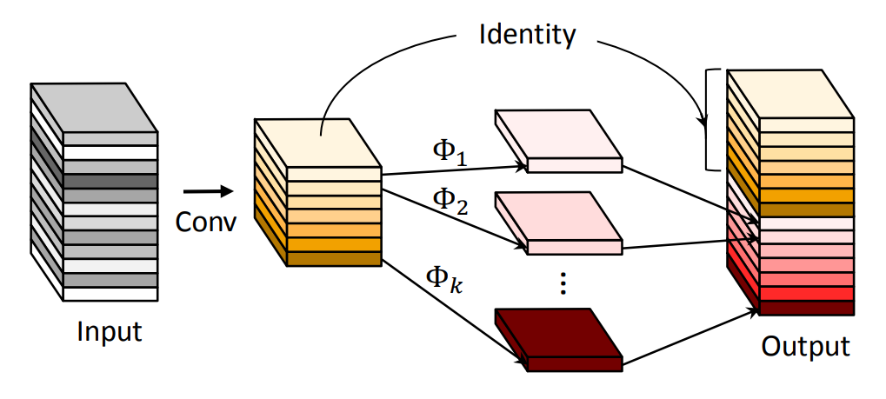
\includegraphics[width = 0.8\textwidth]{ghost卷积.png}
    \caption{ghost卷积示意图}
    \label{ghost1}
\end{figure}

如图\ref{ghost1}所示,ghost模块的做法是用一些更小的卷积核(即参数更少运算更快)替代原先的卷积部分,但是这部分卷积核产生的输出量只能达到相当于本来卷积输出量的一部分,这时根据上文对相似特征图的分析,可以采用一些线性变换的方式去生成剩下的特征图,从而达到用更轻量的卷积滤波器去生成相同规模特征图的目的。

\subsection{基于ghost模块的模型轻量化算法实现}

\begin{figure}[htbp]
    \centering
    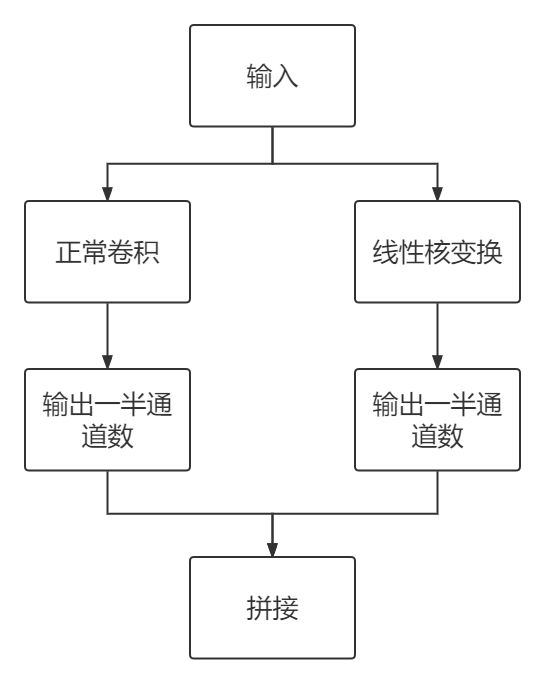
\includegraphics[width = 0.8\textwidth]{ghost算法实现.png}
    \caption{ghost算法实现示意图}
    \label{ghost2}
\end{figure}

本课题的Ghost实现流程如图\ref{ghost2}所示,将原始卷积层改变成两部分,分别产生相当于原始卷积层一半通道数的输出(实际上二者的输出比例可以任意调节),可以使得改进后的模块参数量减少。

\subsection{ghost算法理论分析}

(1)相对于普通卷积模块的加速比

\begin{equation}
    \begin{aligned}
    r_{s} &=\frac{n \cdot h^{\prime} \cdot w^{\prime} \cdot c \cdot k \cdot k}{\frac{n}{s} \cdot h^{\prime} \cdot w^{\prime} \cdot c \cdot k \cdot k+(s-1) \cdot \frac{n}{s} \cdot h^{\prime} \cdot w^{\prime} \cdot d \cdot d} \\
    &=\frac{c \cdot k \cdot k}{\frac{1}{s} \cdot c \cdot k \cdot k+\frac{s-1}{s} \cdot d \cdot d} \approx \frac{s \cdot c}{s+c-1} \approx S
    \end{aligned}
    \label{jsb}
\end{equation}

如式\ref{jsb}所示,设输入通道数为$c$,输出通道数为$n$,输入图像高度为$h^'$和$w^'$,其中保留的原始卷积通道数为本来的$1/s$,原始卷积核大小为$k*k$,线性核大小为$d*d$,由于线性变换是在每个通道上进行,所以代表线性变换的一项中不含输入通道数$c$。

由式\ref{jsb}可得,将原始卷积模块替换为一半卷积一半线性变换的ghost模块后(即将$s=2$代入),可以得到该模块的理论提速比为2。

(1)相对于普通卷积模块的参数压缩比

\begin{equation}
    r_{c}=\frac{n \cdot c \cdot k \cdot k}{\frac{n}{s} \cdot c \cdot k \cdot k+(s-1) \cdot \frac{n}{s} \cdot d \cdot d} \approx \frac{s \cdot c}{s+c-1} \approx \frac{s c}{c}=S
    \label{csys}
\end{equation}

如式\ref{csys}所示,经过计算可以得到改进后的ghost模块和改进之前的普通卷积模块理论参数压缩比为2。

\subsection{ghost算法实验对比分析}
将ghost模块对应改动部署到YOLOv5网络之后,在实验平台上进行测试验证。分别用YOLOv5模块和调整深度之后得到的小型网络(记为YOLOv5s)作为参照,验证YOLOv5+ghost在红外无人机图像数据集上的效果。

\section{轻量化红外无人机目标检测算法嵌入式实现与验证}
为了进一步验证本文提出的轻量化红外无人机目标检测算法的有效性,本节将本文提出的完整算法模型进行转换,并且在嵌入式设备上进行检测和验证。

\subsection{嵌入式设备介绍}

\subsection{tensorrt加速}

\subsection{不同算法性能对比与分析}


